\documentclass[a4paper, 12pt]{article}

\usepackage[left = 1.5cm,
            right = 1.5cm,
            top = 1.5cm,
            bottom = 1.5cm,
            footskip = 0cm]{geometry}
\usepackage{graphicx} % Required for inserting images
\usepackage{wrapfig}

\title{\textbf{Rapport pour le projet de INFOF202}}
\author{
    Ransy Lenny
    \and
    Lejeune Lucas
    }
\date{Janvier 2024}
\renewcommand*\contentsname{Table des matières}

\begin{document}

\maketitle

Ce rapport vise a documenter le projet "Frogger" que nous avons réaliser. Nous traiterons les tâches que nous avons réalisées et comment nous les avons réalisées. Pour cela, nous parlerons des classes que nous avons codées pour faire ce projet, comment elles sont réparties dans le code et comment elles intéragissent entre elles. Nous justifierons aussi comment nous avons utilisé le modèle de conception MVC dans la partie jeu.

\tableofcontents

\pagebreak

\section{Résumé des tâches réalisées et fonctionnement du jeu}
% Résumer comment le jeu marche et listes les tâches réalisées
Nous avons réalisé les tâches principales et toutes les tâches additionnelles, sauf la tâches de l'éditeur de niveau. \\
Ouvrons le jeu et voyons ce qui se passe. 
% Parler du fonctionnement du jeu quand tout sera fini


\section{Structure des fichiers: Utilisation du MVC}
% Parler de l'orga des fichiers

La structure des fichiers peut se diviser en plusieurs parties: les fichiers du jeu, ceux des menus, les mains et les images du jeu. \\

\begin{wrapfigure}{r}{3cm}
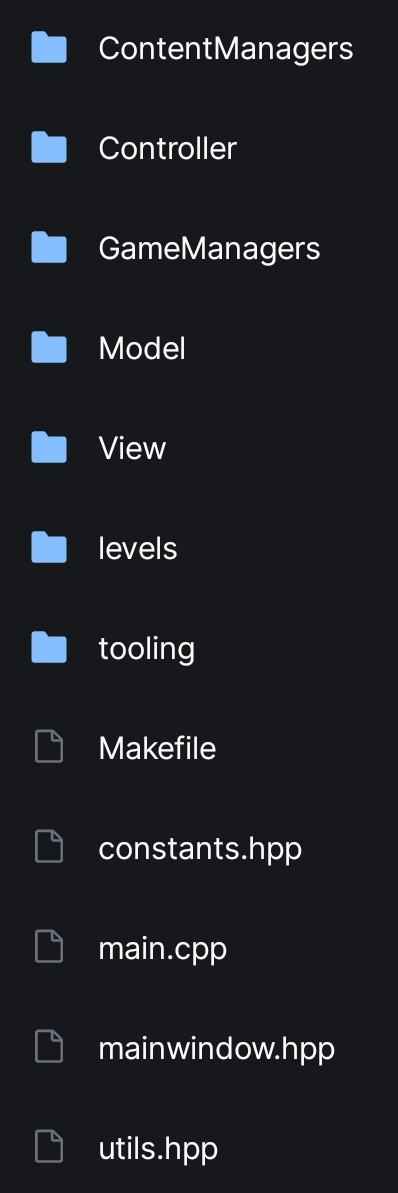
\includegraphics[width=3cm]{Images/folders.jpg}
\end{wrapfigure}

Le dossier \texttt{ContentManagers} contient tout les fichiers de code en rapport avec la gestion des menus du jeu. \\

Les dossiers \texttt{Controller}, \texttt{Model} et \texttt{View} contiennent le code parmettant de faire tourner le jeu (la partie plateau, qui ne compte pas le menu).
Cette disposition met en évidence l'utilisation du MVC. Prenons la gestion de la grenouille comme exemple. 
Les fichiers gérant les contrôles de celle-ci se trouvent dans le dossier \texttt{Controller}, ceux qui gèrent ses propriétés dans le plateau se trouvent dans \texttt{Model} et enfin, ceux qui gèrent son affichage se trouvent dans \texttt{View}. Tout le code de ces fichiers est utilisé dans les fichiers de \texttt{GameManagers} pour avoir un jeu fonctionnel.\\

Le dossier \texttt{levels} contient les données des niveaux sauvegardés en fichiers \texttt{.csv}, et les scores obtenus sur ceux-ci. Plus de détails seront donnés dans les chapitres concernés. \\

Le dossier \texttt{tooling} contient tout les outils construits grâce aux outils venant la librairie FLTK qui sont surtout utilisés dans la partie \texttt{View} et \texttt{ContentManagers}. \\

Le fichiers \texttt{constants.hpp} contient toutes les constantes utilisées dans le projet, comme par exemple la taille des bouttons dans le menu. \\

Enfin, les fichiers \texttt{main.cpp} et \texttt{mainwindow.hpp} s'occupent d'assembler le tout, pour obtenir l'application Frogger au complet.







\section{Fichiers et classes principales}
% Parler des fichiers mains et du gameinit/gameloop.
% Peut-être parler des classes et fichiers principaux pour les menus après?

\section{Réalisation de la base du jeu (Tâches de base)}
% On parle du tout début juste avec les roadlanes

\section{Réalisation des tâches additionnelles}
Maintenant que les tâches principales sont réalisées et que nous avons une bonne base, nous pouvons implémenter les fonctionnalités supplémentaires.

\subsection{Rangées d'eau, buches et tortues}

\subsection{Nénuphars et rangée 13}

\subsection{Vies de la grenouille}

\subsection{Tortues plongeantes}

\subsection{Directions de la grenouille}

\subsection{Score}

\subsection{Meilleur score}

\subsection{Gestion des menus et écran d'accueil}

\subsection{Niveaux et sélection de niveau}

\subsection{Vies}


\end{document}
